\chapter{\MakeUppercase{Technical Specification}}
\justifying

\section{Requirements}

\subsection{Functional Requirements}

To guarantee clinical baseline utility, the system must rigidly fulfil a set of interconnected technical functional requirements. At its core (\textbf{FR-01}), the application must deliver a responsive conversational chat interface specifically dedicated to managing dynamic medical intake interviews. Through this interface (\textbf{FR-02}), it is mandated to seamlessly extract and compile all essential patient data structures---including age, gender profiles, expressed symptoms, the precise 8 diabetes biomarkers, alongside the immediate statuses of requested \ac{ecg} and voice files---relying entirely upon fluid natural language processing rather than static forms. In handling external biomarker data (\textbf{FR-03}), the architecture must robustly support direct file uploads, strictly isolating \ac{ecg} voltage waveform data in CSV format, while parsing audio vocal recordings strictly packaged within WAV, MP3, FLAC, or OGG standards. Once data acquisition is complete, the operational diagnostic pipeline activates: it natively performs cardiac arrhythmia classification (\textbf{FR-04}) through the direct analysis of the ingested \ac{ecg} topology using ECGNet; synchronously computes critical diabetes risk assessments (\textbf{FR-05}) driven by the conversationally mined tabular metrics through DiabetesNet; and strictly evaluates Parkinson's disease motor risk (\textbf{FR-06}) by executing feature extraction on the uploaded voice samples funnelled into ParkinsonNet. Combining these modular evaluations, the system logic (\textbf{FR-07}) must objectively synthesize a unified triage classification state---categorised exclusively as routine, recommended check, or priority review based purely chronologically on combined probabilistic risk escalations. Ultimately, (\textbf{FR-08}), the platform's presentation engine is mandated to render these unified screening results exclusively via clear, highly empathetic, mathematically non-diagnostic prose explicitly generated by the Gemini \ac{llm} handler. Underpinning all these operations (\textbf{FR-09}) exists a strict legal and ethical boundary: the system logic matrix shall fundamentally never generate or infer definitive medical diagnoses; all programmatic or linguistically generated outputs shall be universally and explicitly labelled strictly as preliminary screening results only.

\subsection{Non-Functional Requirements}

To maintain performance and deployability within restricted production environments, strict baseline non-functional execution parameters are enforced. Primarily (\textbf{NFR-01}), inference latency bottlenecks must be systematically bypassed by strictly demanding that all three primary deep learning structures are structurally pre-loaded directly into rapid access memory spaces implicitly at server runtime startup. To prevent sequential request blocking, the asynchronous foundation (\textbf{NFR-02}) heavily delegates all incoming network activity across concurrent FastAPI endpoints. Given the massive reliance on external language interpretation layers, network robustness (\textbf{NFR-03}) relies inherently on implementing a highly resilient Gemini \ac{llm} topological fallback chain---dynamically cascading from the ultra-fast \textit{gemini-1.5-flash}, down to the heavily reasoned \textit{gemini-1.5-pro}, and optionally bottoming at \textit{gemini-2.0-flash}---to fundamentally mitigate standard commercial \ac{api} rate-limiting ceilings. Focusing on user acquisition barriers, the complete frontend experience (\textbf{NFR-04}) must uniformly render successfully natively via any standard commercial web browser architecture completely independent of locally compiled installations or heavy client download packets. On the internal hardware layer (\textbf{NFR-05}), overriding compute boundaries exist declaring that all native operations---ranging strictly from raw deep learning neural inference matrices straight down to sequential digital signal preprocessing topologies---must execute flawlessly strictly upon off-the-shelf CPU hardware architectures, entirely independent of expensive CUDA-enabled GPU hardware clusters. Unifying these structural layers, the backend system (\textbf{NFR-06}) demands absolute operational transmission security governed natively via airtight intra-service \ac{cors} configurations protecting all live \ac{api} session traffic.

\section{Feasibility Study}

\subsection{Technical Feasibility}

All selected technologies are open-source, mature, and freely available. PyTorch $\geq$ 2.0 supports CPU inference without GPU requirements, making the system deployable on standard cloud instances (e.g., Render free tier). The Gemini API offers a free tier sufficient for development and demonstration. FastAPI is production-grade with support for asynchronous I/O. Streamlit provides a modern, interactive frontend with minimal configuration.

The signal processing requirements (Butterworth filtering, R-peak detection, audio feature extraction) are fully addressed by SciPy and librosa, two well-maintained Python libraries.

\subsection{Economic Feasibility}

Development was carried out using free-tier cloud resources (Google Colab T4 GPU for training, Render for deployment) and open-source libraries. The Gemini API's free tier provides sufficient quota for prototype and demonstration usage. No proprietary datasets or paid clinical data sources were required.

\subsection{Operational Feasibility}

The system is deployed as a web application, requiring only a browser and internet connection from the user. Medical data input is guided conversationally by the \ac{llm}, eliminating the need for technical expertise. The explicitly non-diagnostic framing of results ensures the system operates within ethical and regulatory boundaries for a research/educational tool.

\section{System Specifications}

\subsection{Hardware Specifications}

\begin{table}[h!]
\centering
\caption{Hardware Specifications Used for Development and Training}
\renewcommand{\arraystretch}{1.3}
\begin{tabular}{|l|l|l|}
\hline
\textbf{Component} & \textbf{Training (Google Colab)} & \textbf{Deployment (Render Free Tier)} \\
\hline
\ac{cpu} & Intel Xeon (2 vCPUs) & 0.1 vCPU (shared) \\
\ac{gpu} & NVIDIA Tesla T4 (15 GB VRAM) & None (CPU inference) \\
RAM & 12.7 GB & 512 MB \\
Storage & 100 GB (Google Drive) & 1 GB ephemeral \\
\hline
\end{tabular}
\end{table}

\subsection{Software Specifications}

\begin{table}[H]
\centering
\caption{Software Stack and Version Specifications}
\renewcommand{\arraystretch}{1.3}
\begin{tabular}{|l|l|l|}
\hline
\textbf{Component} & \textbf{Software} & \textbf{Version} \\
\hline
Language & Python & 3.10+ \\
\ac{dl} Framework & PyTorch & $\geq$ 2.0.0 \\
Backend \ac{api} & FastAPI & 0.115.0 \\
\ac{api} Server & Uvicorn & 0.30.6 \\
Frontend & Streamlit & 1.38.0 \\
\ac{llm} Client & google-generativeai & $\geq$ 0.8.0 \\
Signal Processing & SciPy & $\geq$ 1.10.0 \\
Audio Processing & librosa & $\geq$ 0.10.0 \\
Data Handling & pandas, NumPy & $\geq$ 2.0.0, $\geq$ 1.24.0 \\
Audio I/O & soundfile & $\geq$ 0.12.0 \\
\ac{ml} Utilities & scikit-learn & $\geq$ 1.3.0 \\
Environment & python-dotenv & $\geq$ 1.0.0 \\
\hline
\end{tabular}
\end{table}

\subsection{Dataset Specifications}

\begin{table}[H]
\centering
\caption{Dataset Specifications for the Three Models}
\renewcommand{\arraystretch}{1.3}
\resizebox{\textwidth}{!}{
\begin{tabular}{|l|l|l|l|l|}
\hline
\textbf{Model} & \textbf{Dataset} & \textbf{Size} & \textbf{Source} & \textbf{Split} \\
\hline
ECGNet & MIT-BIH Arrhythmia Database & 48 records / 109,446 beats & PhysioNet & 28 train / 20 test records \\
DiabetesNet & Pima Indians Diabetes Dataset & 768 samples, 8 features & UCI / NIDDK & 80/20 stratified \\
ParkinsonNet & UCI Parkinson's Dataset & 195 recordings, 22 features & Univ. of Oxford & 80/20 stratified \\
\hline
\end{tabular}}
\end{table}

\section{Model Architecture Specifications}

\subsection{ECGNet — Multi-Scale Attention CNN}

ECGNet processes single-channel \ac{ecg} beat windows of fixed length (252 samples at 360 Hz, corresponding to 0.7 seconds) and classifies each beat into one of five \ac{aami} classes: N (Normal), S (Supraventricular), V (Ventricular), F (Fusion), Q (Paced/Unknown).

The model comprises three Multi-Scale Blocks, each containing three parallel Conv1d layers with kernel sizes 3, 5, and 7, followed by Batch Normalisation, ReLU activation, and a Channel Attention module. The Channel Attention module implements the Squeeze-and-Excitation mechanism:

\begin{equation}
	\hat{x}_{c} = \sigma\!\left(W_2 \cdot \text{ReLU}(W_1 \cdot \text{GAP}(x))\right) \cdot x_c
\end{equation}

where \textit{GAP} denotes Global Average Pooling, $W_1 \in \mathbb{R}^{C/r \times C}$, $W_2 \in \mathbb{R}^{C \times C/r}$ are learnable weights, $r=8$ is the reduction ratio, and \ac{sigma} denotes the sigmoid activation.

The total parameter count is approximately 487K. The model is trained using Focal Loss with $\gamma = 2$:

\begin{equation}
	\mathcal{L}_{\text{focal}} = -\sum_{c} \alpha_c (1 - p_c)^{\gamma} \log(p_c)
\end{equation}

This loss function down-weights easy (common) examples and focuses learning on hard, rare beat classes — an essential property given the severe class imbalance in the MIT-BIH dataset (72\% Normal beats).

\subsection{DiabetesNet — Tabular Deep Neural Network}

DiabetesNet is a three-layer fully connected network operating on 8 StandardScaler-normalised clinical features. The architecture is:

\begin{equation}
	z^{(1)} = \text{BN}(\text{ReLU}(W^{(1)}x + b^{(1)})); \quad \hat{y} = \sigma(W^{(3)}z^{(2)} + b^{(3)})
\end{equation}

where $x \in \mathbb{R}^8$ is the normalised feature vector, and Batch Normalisation (\ac{bn}) with Dropout (rates 0.3 and 0.2) prevents overfitting on the small (768-sample) dataset. Binary cross-entropy with logits loss is used for training:

\begin{equation}
	\mathcal{L}_{\text{BCE}} = -[y \log(\hat{y}) + (1-y) \log(1-\hat{y})]
\end{equation}

\begin{figure}[h!]
\centering
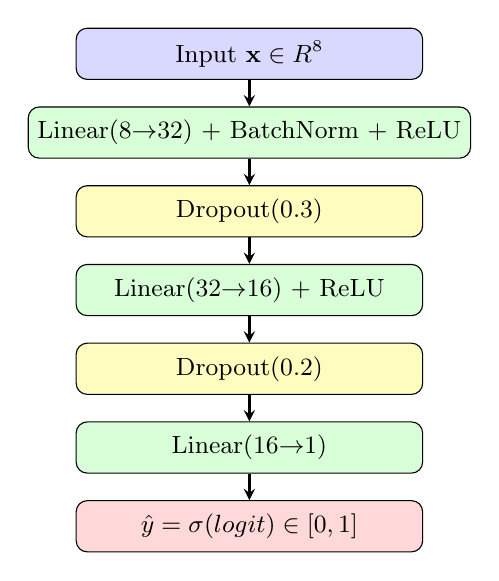
\begin{tikzpicture}[
  node distance=1.0cm,
  box/.style={draw, rounded corners=4pt, minimum width=4.4cm, minimum height=0.65cm,
              text centered, font=\small},
  arrow/.style={->, >=stealth, thick}
]
\node[box, fill=blue!15]   (inp) {Input $\mathbf{x} \in \mathbb{R}^{8}$};
\node[box, fill=green!15,  below of=inp] (l1)  {Linear(8${\to}$32) + BatchNorm + ReLU};
\node[box, fill=yellow!25, below of=l1]  (d1)  {Dropout(0.3)};
\node[box, fill=green!15,  below of=d1]  (l2)  {Linear(32${\to}$16) + ReLU};
\node[box, fill=yellow!25, below of=l2]  (d2)  {Dropout(0.2)};
\node[box, fill=green!15,  below of=d2]  (l3)  {Linear(16${\to}$1)};
\node[box, fill=red!15,    below of=l3]  (out) {$\hat{y} = \sigma(\text{logit}) \in [0,1]$};
\draw[arrow] (inp)--(l1); \draw[arrow] (l1)--(d1); \draw[arrow] (d1)--(l2);
\draw[arrow] (l2)--(d2); \draw[arrow] (d2)--(l3); \draw[arrow] (l3)--(out);
\end{tikzpicture}
\caption[DiabetesNet Architecture]{DiabetesNet Architecture --- Tabular Deep Neural Network (8 $\rightarrow$ 32 $\rightarrow$ 16 $\rightarrow$ 1)}
\label{fig:diabetesnet}
\end{figure}

\subsection{ParkinsonNet — Voice Feature DNN}

ParkinsonNet accepts a 22-dimensional feature vector of acoustic biomarkers extracted from sustained vowel phonation. The architecture mirrors DiabetesNet with higher-capacity layers (22 $\rightarrow$ 64 $\rightarrow$ 32 $\rightarrow$ 1) and stronger regularisation (Dropout 0.4). The 22 features span fundamental frequency statistics, jitter, shimmer, noise ratios, nonlinear dynamics, and pitch entropy measures, all normalised using StandardScaler fitted to the UCI training set.

\begin{figure}[h!]
\centering
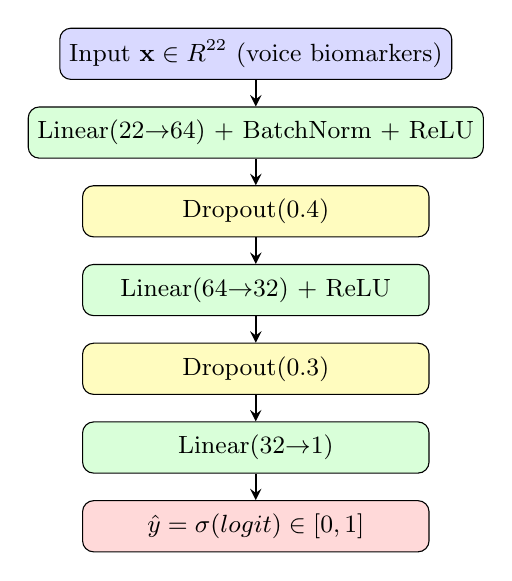
\begin{tikzpicture}[
  node distance=1.0cm,
  box/.style={draw, rounded corners=4pt, minimum width=4.4cm, minimum height=0.65cm,
              text centered, font=\small},
  arrow/.style={->, >=stealth, thick}
]
\node[box, fill=blue!15]   (inp) {Input $\mathbf{x} \in \mathbb{R}^{22}$ (voice biomarkers)};
\node[box, fill=green!15,  below of=inp] (l1)  {Linear(22${\to}$64) + BatchNorm + ReLU};
\node[box, fill=yellow!25, below of=l1]  (d1)  {Dropout(0.4)};
\node[box, fill=green!15,  below of=d1]  (l2)  {Linear(64${\to}$32) + ReLU};
\node[box, fill=yellow!25, below of=l2]  (d2)  {Dropout(0.3)};
\node[box, fill=green!15,  below of=d2]  (l3)  {Linear(32${\to}$1)};
\node[box, fill=red!15,    below of=l3]  (out) {$\hat{y} = \sigma(\text{logit}) \in [0,1]$};
\draw[arrow] (inp)--(l1); \draw[arrow] (l1)--(d1); \draw[arrow] (d1)--(l2);
\draw[arrow] (l2)--(d2); \draw[arrow] (d2)--(l3); \draw[arrow] (l3)--(out);
\end{tikzpicture}
\caption[ParkinsonNet Architecture]{ParkinsonNet Architecture --- Voice Feature Deep Neural Network (22 $\rightarrow$ 64 $\rightarrow$ 32 $\rightarrow$ 1)}
\label{fig:parkinsonnet}
\end{figure}

\section{API Specification}

\begin{table}[h!]
\centering
\caption{FastAPI Endpoint Specifications}
\renewcommand{\arraystretch}{1.3}
\begin{tabular}{|l|l|>{\raggedright\arraybackslash}p{5.5cm}|>{\raggedright\arraybackslash}p{5cm}|}
\hline
\textbf{Endpoint} & \textbf{Method} & \textbf{Input} & \textbf{Output} \\
\hline
\texttt{/chat} & POST & \texttt{ChatRequest} (messages, file paths) & \texttt{ChatResponse} (response, model\_results) \\
\texttt{/upload} & POST & Multipart file (CSV or WAV) & \texttt{UploadResponse} (file\_path, type) \\
\texttt{/health} & GET & None & Health status JSON \\
\texttt{/} & GET & None & API status JSON \\
\hline
\end{tabular}
\end{table}
